\section{Introduction}\label{Introduction}

3D scene reconstruction aims to recover scene geometry and appearance from multi-view observations and is essential for applications such as autonomous driving, AR/VR, robotic perception, and digital twins. In indoor navigation, accurate and efficient 3D modeling is crucial for spatial perception and localization. Prior research has explored robust sensing and efficient inference in complex environments~\cite{Knowledge-based,Nonconvex,Cost-Effective}, highlighting the importance of balancing accuracy, robustness, and computational efficiency.

Multi-View Stereo (MVS) achieves high-precision reconstruction via multi-view matching and depth estimation, but performance degrades under low-texture conditions. Neural Radiance Fields (NeRF)~\cite{nerf} improve view synthesis but require dense inputs and per-scene optimization. For efficient inference, explicit 3D Gaussian Splatting (3DGS)~\cite{3DGS} represents scenes with Gaussian ellipsoids, enabling fast rendering and gradient-based optimization. Following this approach, feed-forward variants~\cite{pixelsplat,mvsplat} improve inference efficiency and generalization through end-to-end prediction, while still often struggling to maintain geometric consistency. In contrast, optimization-based methods, such as VCR-GauS~\cite{vcr} and NeuSG~\cite{neusg}, incorporate geometric priors and normal constraints to refine scene structure, achieving higher accuracy at the cost of efficiency and generalization.

With the increasing adoption of panoramic cameras, 360 images have become an effective source for sparse-view reconstruction~\cite{wu2023360}, capturing the entire scene in a single shot. Feed-forward panoramic methods focus on rendering quality, but projection distortions and unstable depth estimation often cause structural drift, limiting faithful geometric recovery.

To address these challenges, we propose 360-GeoGS, a feed-forward 3DGS framework for 360 image inputs that incorporates Depth-Normal (D-Normal) regularization. The framework predicts multi-view depth from 360 images and fuses various features, which are then processed by a U-Net to regress pixel-aligned Gaussian primitives. D-Normal regularization is applied in the rendering space to jointly supervise Gaussian position, scale, and orientation. Experiments on multiple panoramic benchmarks demonstrate that our method substantially improves geometric consistency and surface continuity while maintaining high rendering quality, outperforming existing feed-forward panoramic 3DGS methods. Our main contributions are as follows:
\begin{figure*}[ht!]
\captionsetup{justification=raggedright,singlelinecheck=false}
\begin{center}
	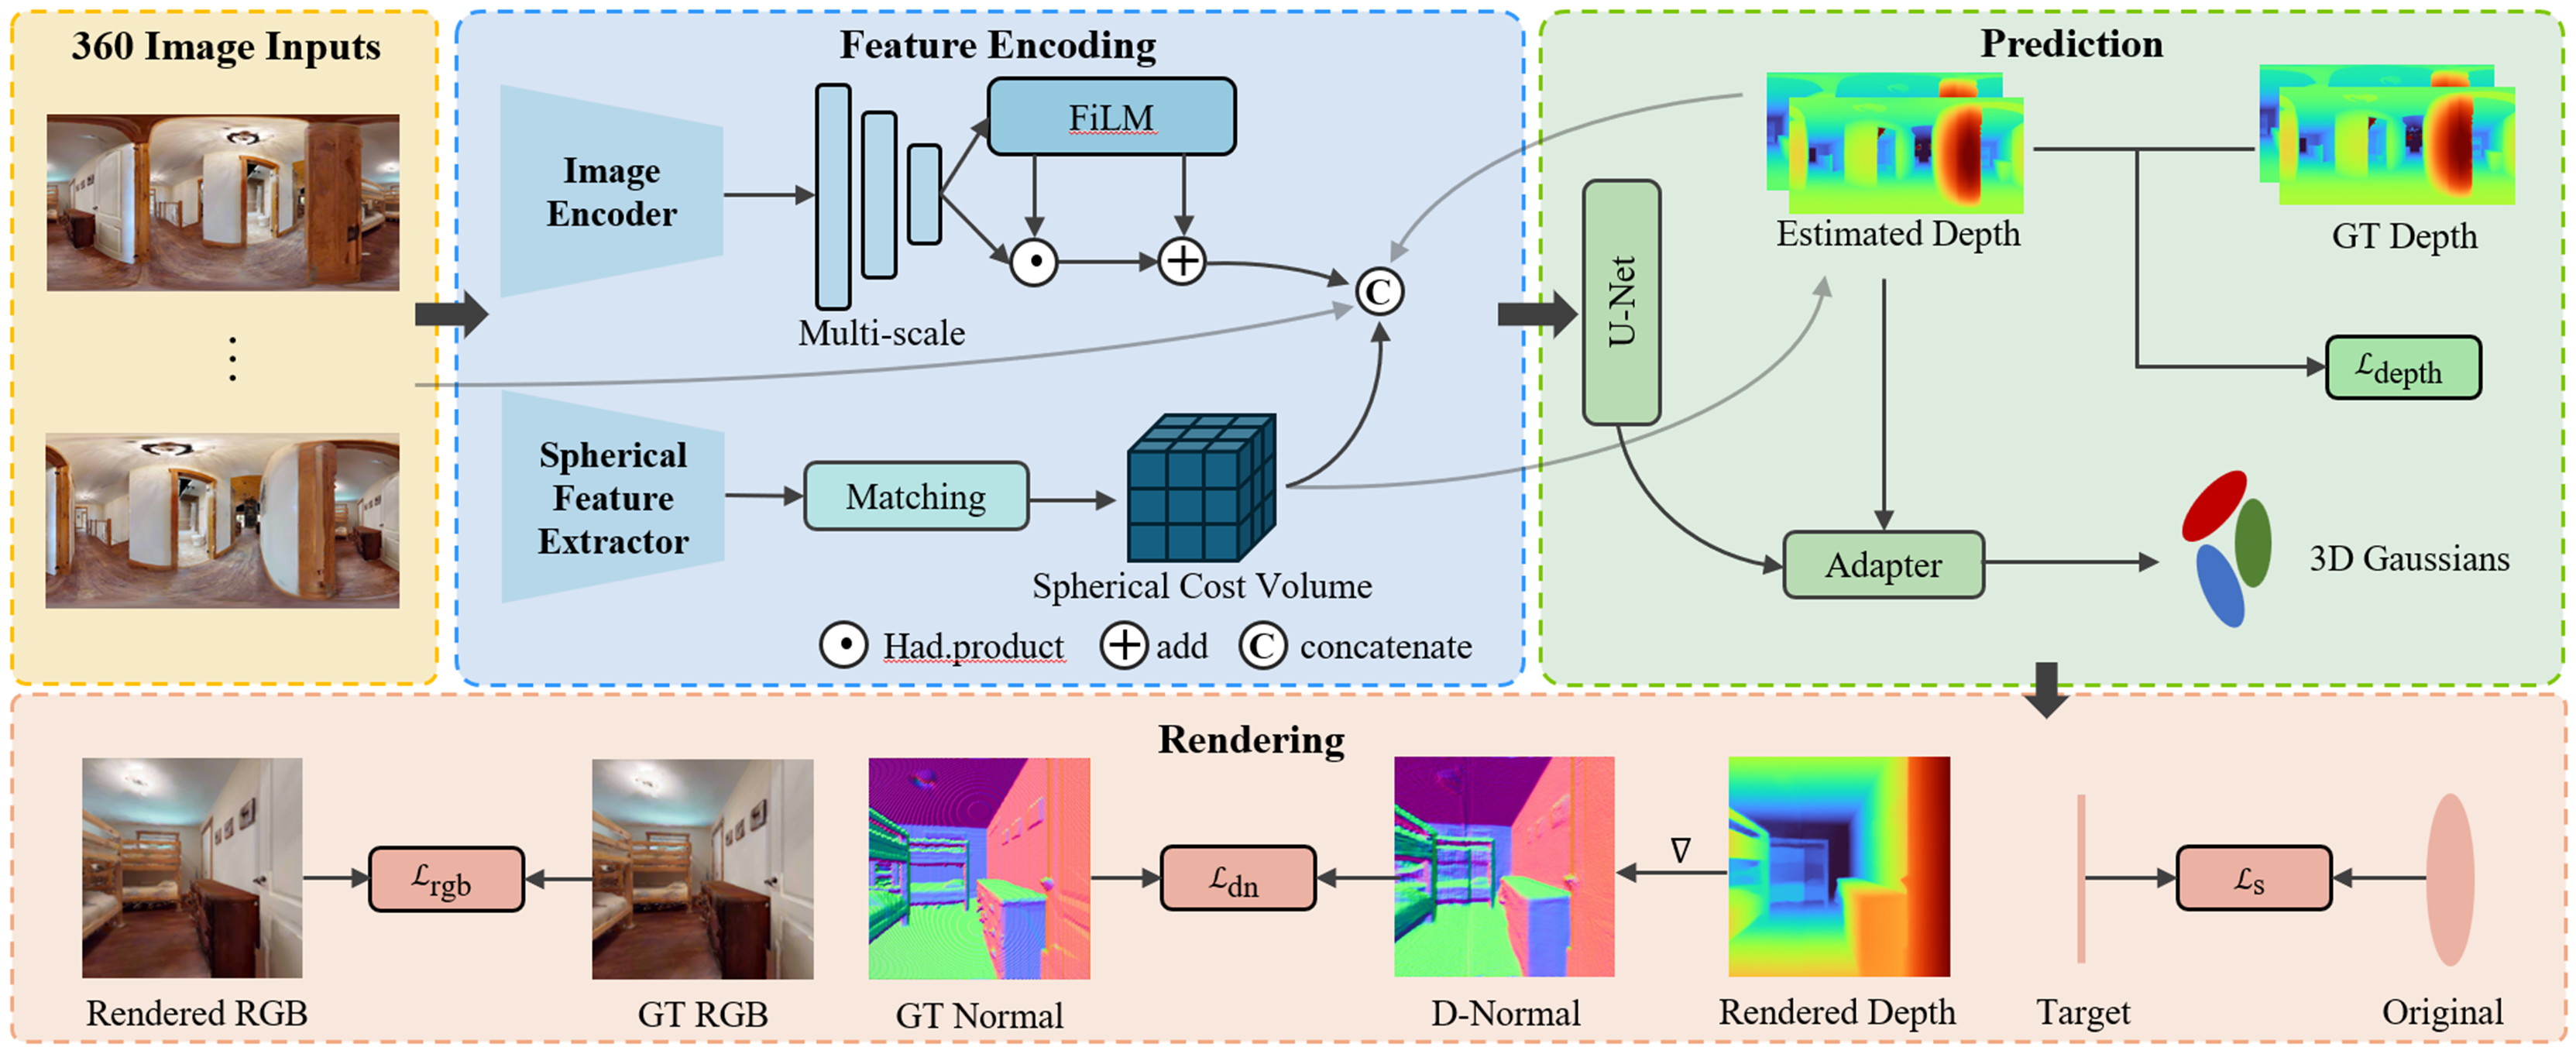
\includegraphics[width=1.0\textwidth]{figures/small_pipline.png}
	\caption{Our pipeline extracts matching features from 360 images using a SphereCNN to construct a spherical cost volume and regress initial depth. Multi-scale features are also extracted by an image encoder and modulated via a FiLM module. The spherical cost volume, modulated multi-scale features, initial RGB images, and depth estimates are then fused to form a unified multi-modal representation, which is decoded by a U-Net and further refined by an adapter to produce per-pixel 3D Gaussian parameters. The network is trained with four losses: $\mathcal{L}_{\mathrm{rgb}}$, $\mathcal{L}_\mathrm{s}$, $\mathcal{L}_{\mathrm{dn}}$, and $\mathcal{L}_{\mathrm{depth}}$ (the definitions of $\mathcal{L}_\mathrm{s}$ and $\mathcal{L}_{\mathrm{dn}}$ are provided in Section~\ref{subsec:D-Normal}).}
\label{fig:pipeline}
\end{center}
\end{figure*}
\begin{enumerate}
\item We propose a feed-forward 3DGS network for 360 image inputs, which employs a SphereCNN backbone to extract spherical features and build a spherical cost volume for depth estimation. Based on the estimated depth, the network performs feed-forward inference to rapidly predict 3D Gaussian parameters, achieving efficient and accurate 3D scene reconstruction.
\item We introduce D-Normal regularization, which jointly optimizes surface normals and Gaussian positions to ensure that neighboring Gaussian primitives form coherent local surfaces with consistent orientation and spatial alignment, thereby enhancing the geometric consistency and accuracy of the predicted 3DGS points.
\item Extensive experiments across multiple benchmarks demonstrate that our approach delivers superior geometric performance while preserving high rendering quality.
\end{enumerate}

